\documentclass[11pt,a4paper]{article}
\usepackage[utf8]{inputenc}
\usepackage[T1]{fontenc}
\usepackage{geometry}
\usepackage{graphicx}
\usepackage{amsmath}
\usepackage{amssymb}
\usepackage{listings}
\usepackage{xcolor}
\usepackage{hyperref}
\usepackage{booktabs}
\usepackage{float}
\usepackage{caption}
\usepackage{subcaption}
\usepackage{tikz}
\usetikzlibrary{shapes,arrows,positioning,calc,decorations.pathmorphing,decorations.markings,patterns}

\geometry{margin=1in}

\title{Airborne AALIS: Acoustic Drone Detection System\\
Design Document for Drone-Mounted Implementation}
\author{AALIS Development Team}
\date{\today}

\hypersetup{
    colorlinks=true,
    linkcolor=blue,
    filecolor=magenta,      
    urlcolor=cyan,
    pdftitle={Airborne AALIS Design Document},
}

\definecolor{codegreen}{rgb}{0,0.6,0}
\definecolor{codegray}{rgb}{0.5,0.5,0.5}
\definecolor{codepurple}{rgb}{0.58,0,0.82}
\definecolor{backcolour}{rgb}{0.95,0.95,0.92}

\lstdefinestyle{mystyle}{
    backgroundcolor=\color{backcolour},   
    commentstyle=\color{codegreen},
    keywordstyle=\color{magenta},
    numberstyle=\tiny\color{codegray},
    stringstyle=\color{codepurple},
    basicstyle=\ttfamily\footnotesize,
    breakatwhitespace=false,         
    breaklines=true,                 
    captionpos=b,                    
    keepspaces=true,                 
    numbers=left,                    
    numbersep=5pt,                  
    showspaces=false,                
    showstringspaces=false,
    showtabs=false,                  
    tabsize=2
}

\lstset{style=mystyle}

\begin{document}

\maketitle

\begin{abstract}
This document presents a comprehensive design for mounting the AALIS (Acoustic Autonomous Lightweight Interception System) on an unmanned aerial vehicle (UAV). The airborne implementation enables mobile, real-time acoustic detection of other drones, creating a counter-drone capability or enabling collaborative drone operations. This design addresses the unique challenges of acoustic detection in a noisy airborne environment, including self-noise cancellation, power constraints, weight limitations, and real-time processing requirements.
\end{abstract}

\tableofcontents
\newpage

\section{Executive Summary}

The Airborne AALIS system extends the ground-based acoustic drone detection platform to operate on a host drone platform. This enables:

\begin{itemize}
    \item \textbf{Mobile Detection}: Detection capability that moves with the host platform
    \item \textbf{Counter-Drone Operations}: Active detection and tracking of hostile or unauthorized drones
    \item \textbf{Collaborative Operations}: Detection and identification of friendly drones for coordination
    \item \textbf{Extended Range}: Detection from elevated positions with reduced ground clutter interference
    \item \textbf{Rapid Deployment}: Quick positioning of detection assets to areas of interest
\end{itemize}

The primary technical challenge is distinguishing target drone acoustic signatures from the host drone's own noise, requiring sophisticated self-noise cancellation and adaptive filtering techniques.

\section{System Architecture}

\subsection{High-Level Architecture}

The Airborne AALIS system consists of three primary subsystems:

\begin{enumerate}
    \item \textbf{Acoustic Sensor Array}: Multiple microphones positioned to maximize target detection while minimizing host noise interference
    \item \textbf{Processing Unit}: Embedded computing system for real-time signal processing and classification
    \item \textbf{Communication Module}: Data link for transmitting detection results and receiving commands
\end{enumerate}

\begin{figure}[H]
\centering
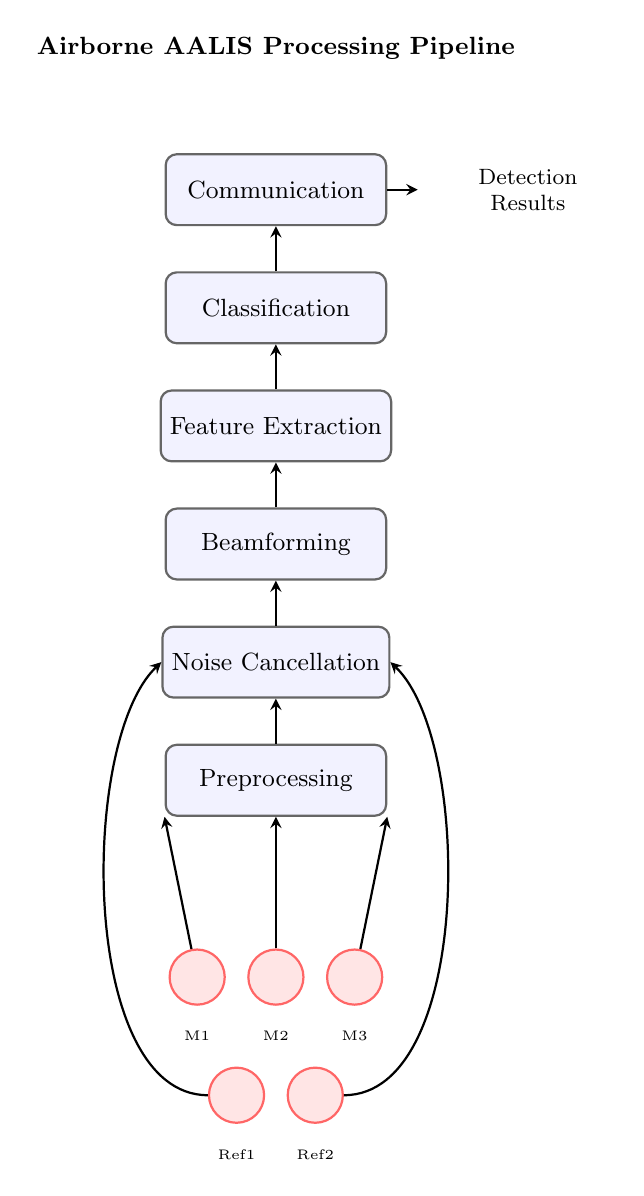
\begin{tikzpicture}[
    block/.style={rectangle, draw=black!60, fill=blue!5, thick, minimum width=2.8cm, minimum height=0.9cm, text centered, rounded corners, font=\small},
    sensor/.style={circle, draw=red!60, fill=red!10, thick, minimum size=0.7cm},
    arrow/.style={->, >=stealth, thick},
    label/.style={text width=2cm, text centered, font=\footnotesize}
]
    % Sensors (spaced out more)
    \node[sensor] (mic1) at (-1,0) {};
    \node[sensor] (mic2) at (0,0) {};
    \node[sensor] (mic3) at (1,0) {};
    \node[sensor] (ref1) at (-0.5,-1.5) {};
    \node[sensor] (ref2) at (0.5,-1.5) {};
    
    \node[below of=mic1, yshift=0.25cm, font=\tiny] {M1};
    \node[below of=mic2, yshift=0.25cm, font=\tiny] {M2};
    \node[below of=mic3, yshift=0.25cm, font=\tiny] {M3};
    \node[below of=ref1, yshift=0.25cm, font=\tiny] {Ref1};
    \node[below of=ref2, yshift=0.25cm, font=\tiny] {Ref2};
    
    % Processing blocks (more spacing)
    \node[block] (preproc) at (0,2.5) {Preprocessing};
    \node[block] (cancel) at (0,4.0) {Noise Cancellation};
    \node[block] (beam) at (0,5.5) {Beamforming};
    \node[block] (features) at (0,7.0) {Feature Extraction};
    \node[block] (classify) at (0,8.5) {Classification};
    \node[block] (comm) at (0,10.0) {Communication};
    
    % Arrows from sensors (straight vertical paths to bottom of preprocessing box)
    \draw[arrow] (mic1) -- (preproc.south west);
    \draw[arrow] (mic2) -- (preproc.south);
    \draw[arrow] (mic3) -- (preproc.south east);
    % Reference arrows go around the outside
    \draw[arrow] (ref1) .. controls (-2.5,-1.5) and (-2.5,3.0) .. (cancel.west);
    \draw[arrow] (ref2) .. controls (2.5,-1.5) and (2.5,3.0) .. (cancel.east);
    
    % Processing flow arrows
    \draw[arrow] (preproc) -- (cancel);
    \draw[arrow] (cancel) -- (beam);
    \draw[arrow] (beam) -- (features);
    \draw[arrow] (features) -- (classify);
    \draw[arrow] (classify) -- (comm);
    
    % Output
    \node[right of=comm, xshift=2.2cm, label] {Detection Results};
    \draw[arrow] (comm) -- ++(1.8,0);
    
    % Title
    \node[above of=comm, yshift=0.8cm, font=\bfseries\small] {Airborne AALIS Processing Pipeline};
\end{tikzpicture}
\caption{High-level architecture of Airborne AALIS system}
\label{fig:architecture}
\end{figure}

\subsection{Physical Integration}

\subsubsection{Sensor Placement}

\begin{figure}[H]
\centering
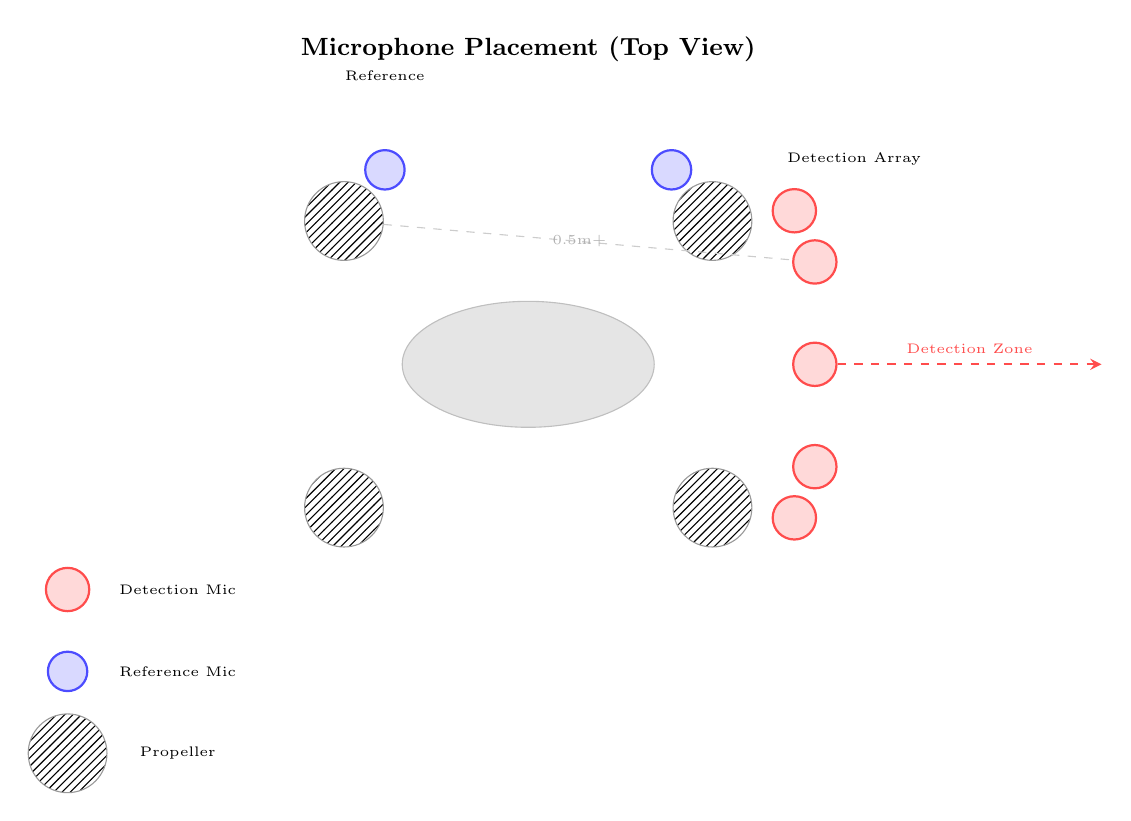
\begin{tikzpicture}[
    scale=1.3,
    drone body/.style={ellipse, draw=gray!50, fill=gray!20, minimum width=3.2cm, minimum height=1.6cm},
    prop/.style={circle, draw=black!40, fill=black!10, minimum size=1.0cm, pattern=north east lines},
    mic/.style={circle, draw=red!70, fill=red!15, thick, minimum size=0.55cm},
    ref mic/.style={circle, draw=blue!70, fill=blue!15, thick, minimum size=0.5cm},
    arrow/.style={->, >=stealth, thick, dashed, gray!50},
    label/.style={font=\tiny}
]
    % Drone body (top view)
    \node[drone body] (body) at (0,0) {};
    
    % Propellers (more spacing - moved further from center)
    \node[prop] (prop1) at (-1.8,1.4) {};
    \node[prop] (prop2) at (1.8,1.4) {};
    \node[prop] (prop3) at (-1.8,-1.4) {};
    \node[prop] (prop4) at (1.8,-1.4) {};
    
    % Detection microphones (forward-facing array, much better spaced)
    \node[mic] (mic1) at (2.8,1.0) {};
    \node[mic] (mic2) at (2.8,0) {};
    \node[mic] (mic3) at (2.8,-1.0) {};
    \node[mic] (mic4) at (2.6,1.5) {};
    \node[mic] (mic5) at (2.6,-1.5) {};
    
    % Reference microphones (near propellers, more spacing - moved further from propellers)
    \node[ref mic] (ref1) at (-1.4,1.9) {};
    \node[ref mic] (ref2) at (1.4,1.9) {};
    
    % Labels (positioned to avoid overlap)
    \node[label, above of=mic1, yshift=0.3cm, xshift=0.5cm] {Detection Array};
    \node[label, above of=ref1, yshift=0.2cm] {Reference};
    
    % Detection zone arrow (longer, clearer)
    \draw[arrow, red!70] (mic2) -- ++(2.8,0) node[midway, above, font=\tiny] {Detection Zone};
    
    % Distance indicators (clearer positioning - adjusted for new positions)
    \draw[dashed, gray!40] (prop1) -- (mic1);
    \node[font=\tiny, gray!60] at (0.5,1.2) {0.5m+};
    
    % Title (more space)
    \node[above of=body, yshift=3.0cm, font=\bfseries\small] {Microphone Placement (Top View)};
    
    % Legend (better positioned with text labels and more spacing)
    \node[mic] (legmic) at (-4.5,-2.2) {};
    \node[label, right of=legmic, xshift=0.4cm] {Detection Mic};
    \node[ref mic] (legref) at (-4.5,-3.0) {};
    \node[label, right of=legref, xshift=0.4cm] {Reference Mic};
    \node[prop] (legprop) at (-4.5,-3.8) {};
    \node[label, right of=legprop, xshift=0.4cm] {Propeller};
\end{tikzpicture}
\caption{Optimal microphone placement on host drone platform}
\label{fig:placement}
\end{figure}

Optimal microphone placement requires careful consideration:

\begin{itemize}
    \item \textbf{Forward-facing array}: Primary detection zone ahead of host drone
    \item \textbf{Isolation from propellers}: Maximum distance from host drone propellers (minimum 0.5m recommended)
    \item \textbf{Wind protection}: Acoustic windshields or foam covers to reduce wind noise
    \item \textbf{Multiple positions}: Arrays at different locations to enable beamforming and noise cancellation
\end{itemize}

Recommended configuration:
\begin{itemize}
    \item 4-6 microphones in forward-facing array
    \item 2 reference microphones near propellers for self-noise measurement
    \item All microphones with omnidirectional or cardioid patterns
    \item Frequency response: 50 Hz - 20 kHz
    \item Dynamic range: 40-120 dB SPL
\end{itemize}

\subsubsection{Weight and Power Budget}

Typical weight allocation for small to medium UAV (5-25 kg):

\begin{table}[H]
\centering
\begin{tabular}{lr}
\toprule
\textbf{Component} & \textbf{Weight (g)} \\
\midrule
Microphone array (6 units) & 60-120 \\
Processing unit & 200-500 \\
Power supply/battery & 300-800 \\
Mounting hardware & 100-200 \\
Cabling & 50-100 \\
\hline
\textbf{Total} & \textbf{710-1720} \\
\bottomrule
\end{tabular}
\caption{Weight budget for Airborne AALIS components}
\label{tab:weight}
\end{table}

Power consumption estimates:

\begin{table}[H]
\centering
\begin{tabular}{lr}
\toprule
\textbf{Component} & \textbf{Power (W)} \\
\midrule
Microphones (6 units) & 0.06-0.12 \\
Processing unit (idle) & 2-5 \\
Processing unit (active) & 8-15 \\
Communication module & 1-3 \\
\hline
\textbf{Total (active)} & \textbf{9-18} \\
\bottomrule
\end{tabular}
\caption{Power consumption estimates}
\label{tab:power}
\end{table}

\section{Signal Processing Architecture}

\subsection{Self-Noise Cancellation}

The fundamental challenge is separating target drone signatures from host drone noise. This requires a multi-stage approach:

\subsubsection{Reference-Based Cancellation}

\begin{figure}[H]
\centering
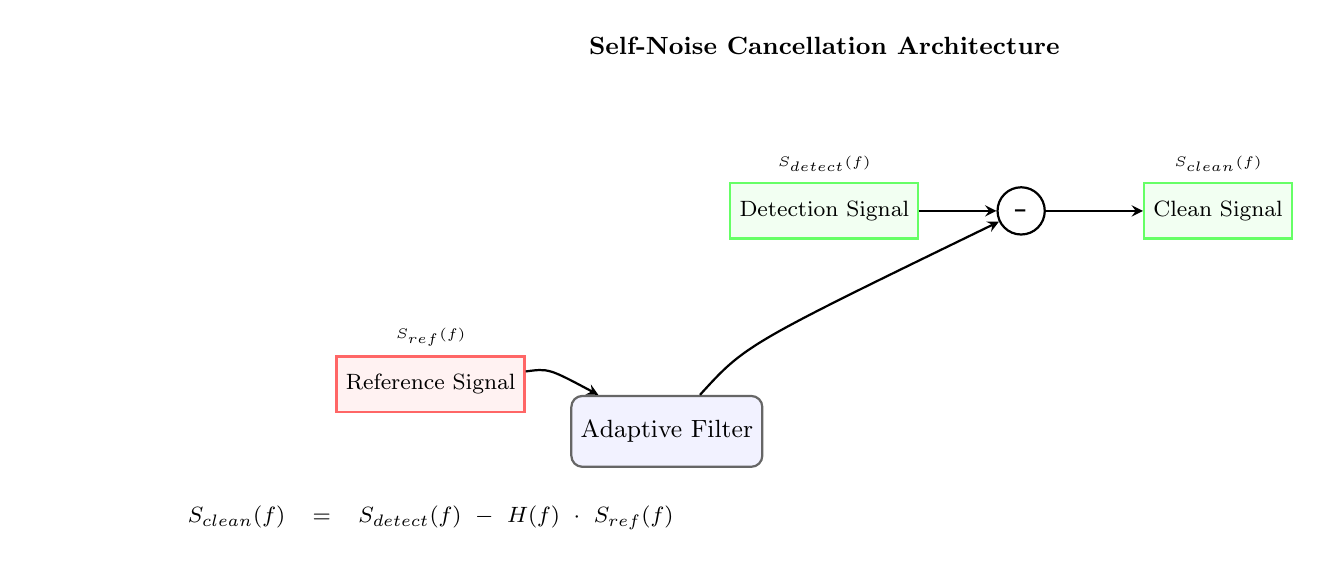
\begin{tikzpicture}[
    block/.style={rectangle, draw=black!60, fill=blue!5, thick, minimum width=2.2cm, minimum height=0.9cm, text centered, rounded corners, font=\small},
    signal/.style={rectangle, draw=green!60, fill=green!5, thick, minimum width=1.8cm, minimum height=0.7cm, text centered, font=\footnotesize},
    noise/.style={rectangle, draw=red!60, fill=red!5, thick, minimum width=1.8cm, minimum height=0.7cm, text centered, font=\footnotesize},
    arrow/.style={->, >=stealth, thick},
    minus/.style={circle, draw=black, thick, minimum size=0.6cm, label={[font=\Large]center:-}}
]
    % Input signals (better spacing)
    \node[signal] (detect) at (0,2.0) {Detection Signal};
    \node[noise] (ref) at (-5.0,-0.2) {Reference Signal};
    
    % Adaptive filter (more space from reference - moved further right and slightly down)
    \node[block] (filter) at (-2.0,-0.8) {Adaptive Filter};
    
    % Summation (more space)
    \node[minus] (sum) at (2.5,2.0) {};
    
    % Output
    \node[signal] (output) at (5.0,2.0) {Clean Signal};
    
    % Arrows (clearer paths - adjusted for new positions with curved paths)
    \draw[arrow] (detect) -- (sum);
    \draw[arrow] (ref) .. controls (-3.5,0.0) .. (filter);
    \draw[arrow] (filter) .. controls (-1.0,0.3) .. (sum);
    \draw[arrow] (sum) -- (output);
    
    % Labels (positioned to avoid overlap)
    \node[above of=detect, yshift=-0.4cm, font=\tiny] {$S_{detect}(f)$};
    \node[above of=ref, yshift=-0.4cm, font=\tiny] {$S_{ref}(f)$};
    \node[above of=output, yshift=-0.4cm, font=\tiny] {$S_{clean}(f)$};
    
    % Title (more space)
    \node[above of=detect, yshift=1.1cm, font=\bfseries\small] {Self-Noise Cancellation Architecture};
    
    % Note (better positioned)
    \node[below of=ref, yshift=-0.7cm, font=\footnotesize, text width=10cm, text centered] {
        $S_{clean}(f) = S_{detect}(f) - H(f) \cdot S_{ref}(f)$
    };
\end{tikzpicture}
\caption{Reference-based noise cancellation system}
\label{fig:cancellation}
\end{figure}

\begin{enumerate}
    \item \textbf{Reference Microphones}: Positioned near host propellers to capture self-noise characteristics
    \item \textbf{Adaptive Filtering}: Use reference signals to predict and subtract host noise from detection microphones
    \item \textbf{Frequency-Domain Processing}: Apply cancellation in frequency domain where noise characteristics are more stable
\end{enumerate}

The cancellation algorithm:

\begin{equation}
S_{clean}(f) = S_{detect}(f) - H(f) \cdot S_{ref}(f)
\end{equation}

Where:
\begin{itemize}
    \item $S_{clean}(f)$: Cleaned signal spectrum
    \item $S_{detect}(f)$: Detection microphone spectrum
    \item $S_{ref}(f)$: Reference microphone spectrum
    \item $H(f)$: Adaptive transfer function (updated continuously)
\end{itemize}

\subsubsection{Beamforming}

\begin{figure}[H]
\centering
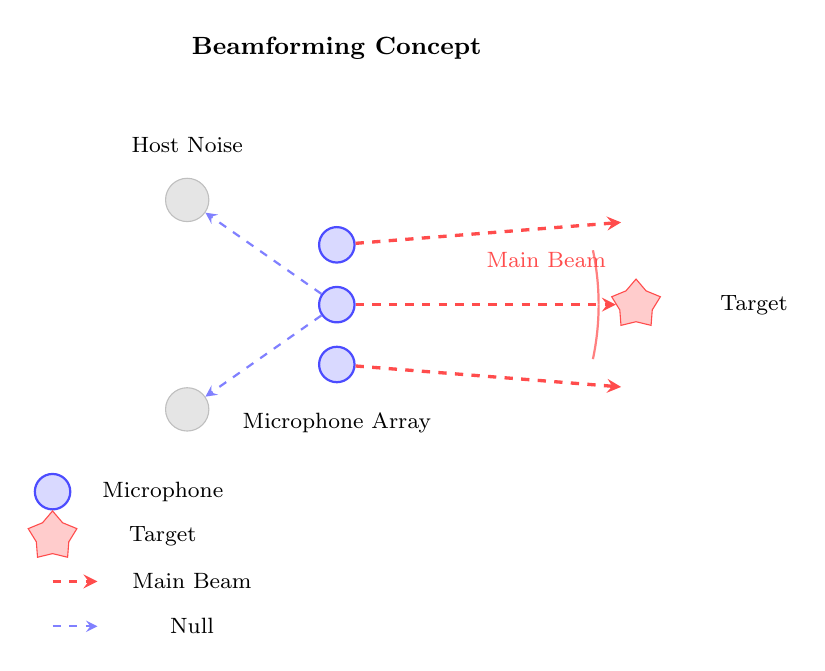
\begin{tikzpicture}[
    scale=0.95,
    mic/.style={circle, draw=blue!70, fill=blue!15, thick, minimum size=0.45cm},
    target/.style={star, star points=5, draw=red!70, fill=red!20, minimum size=0.65cm},
    beam/.style={->, >=stealth, very thick, red!70, dashed},
    null/.style={->, >=stealth, thick, blue!50, dashed},
    label/.style={font=\footnotesize}
]
    % Microphone array (more spacing)
    \node[mic] (mic1) at (0,0.8) {};
    \node[mic] (mic2) at (0,0) {};
    \node[mic] (mic3) at (0,-0.8) {};
    
    % Target direction (more space)
    \node[target] (target) at (4.0,0) {};
    
    % Host propellers (noise sources, better positioned)
    \node[circle, draw=gray!50, fill=gray!20, minimum size=0.55cm] (noise1) at (-2.0,1.4) {};
    \node[circle, draw=gray!50, fill=gray!20, minimum size=0.55cm] (noise2) at (-2.0,-1.4) {};
    
    % Beam pattern (main lobe, clearer)
    \draw[beam] (mic2) -- (target);
    \draw[beam] (mic1) -- ++(3.8,0.3);
    \draw[beam] (mic3) -- ++(3.8,-0.3);
    
    % Null directions (clearer)
    \draw[null] (mic2) -- (noise1);
    \draw[null] (mic2) -- (noise2);
    
    % Labels (better positioned)
    \node[label, right of=target, xshift=0.5cm] {Target};
    \node[label, above of=noise1, yshift=-0.3cm] {Host Noise};
    \node[label, below of=mic2, yshift=-0.5cm] {Microphone Array};
    
    % Beam pattern arc (clearer)
    \draw[red!50, thick] (mic2) ++(0:3.5cm) arc (0:12:3.5cm);
    \draw[red!50, thick] (mic2) ++(0:3.5cm) arc (0:-12:3.5cm);
    \node[label, red!70] at (2.8,0.6) {Main Beam};
    
    % Title (more space)
    \node[above of=mic1, yshift=1.5cm, font=\bfseries\small] {Beamforming Concept};
    
    % Legend (better positioned with text labels and more space above)
    \node[mic] (legmic) at (-3.8,-2.5) {};
    \node[label, right of=legmic, xshift=0.4cm] {Microphone};
    \node[target] (legtarg) at (-3.8,-3.1) {};
    \node[label, right of=legtarg, xshift=0.4cm] {Target};
    \coordinate (legbeamstart) at (-3.8,-3.7);
    \coordinate (legbeamend) at (-3.2,-3.7);
    \draw[beam] (legbeamstart) -- (legbeamend);
    \node[label, right of=legbeamend, xshift=0.2cm] {Main Beam};
    \coordinate (legnullstart) at (-3.8,-4.3);
    \coordinate (legnullend) at (-3.2,-4.3);
    \draw[null] (legnullstart) -- (legnullend);
    \node[label, right of=legnullend, xshift=0.2cm] {Null};
\end{tikzpicture}
\caption{Beamforming for spatial filtering and noise rejection}
\label{fig:beamforming}
\end{figure}

Use microphone array to spatially filter signals:

\begin{itemize}
    \item \textbf{Delay-and-sum beamforming}: Focus on forward direction
    \item \textbf{Null steering}: Create nulls in directions of host propellers
    \item \textbf{Adaptive beamforming}: Adjust beam pattern based on detected noise sources
\end{itemize}

\subsubsection{Host RPM Compensation}

\begin{itemize}
    \item Monitor host drone motor RPM via flight controller telemetry
    \item Predict expected noise frequencies: $f_{noise} = RPM \times blades / 60$
    \item Apply notch filters at predicted frequencies
    \item Adaptively adjust filter bandwidth based on RPM stability
\end{itemize}

\subsection{Enhanced Feature Extraction}

Modify feature extraction to account for airborne environment:

\begin{itemize}
    \item \textbf{Doppler compensation}: Account for relative motion between host and target
    \item \textbf{Altitude normalization}: Adjust frequency response based on air density
    \item \textbf{Wind filtering}: Enhanced temporal filtering to remove wind noise artifacts
    \item \textbf{Motion compensation}: Use IMU data to compensate for host platform motion
\end{itemize}

\subsection{Adaptive Classification}

\begin{itemize}
    \item \textbf{Context-aware thresholds}: Adjust detection thresholds based on:
    \begin{itemize}
        \item Host drone RPM (higher RPM = higher noise floor)
        \item Altitude (affects sound propagation)
        \item Wind conditions
        \item Host platform velocity
    \end{itemize}
    \item \textbf{Dynamic prototype weighting}: Weight prototypes differently based on:
    \begin{itemize}
        \item Expected frequency shifts due to Doppler effect
        \item Altitude-dependent propagation characteristics
        \item Relative velocity estimates
    \end{itemize}
\end{itemize}

\section{Hardware Requirements}

\subsection{Processing Unit}

Requirements for real-time processing:

\begin{itemize}
    \item \textbf{CPU}: ARM Cortex-A78 or equivalent (4+ cores, 2+ GHz)
    \item \textbf{RAM}: Minimum 4 GB (8 GB recommended)
    \item \textbf{Storage}: 32+ GB eMMC or SSD for prototype library and buffering
    \item \textbf{Interfaces}:
    \begin{itemize}
        \item Multiple I2S interfaces for microphone arrays
        \item SPI/UART for flight controller communication
        \item Ethernet/WiFi for data transmission
        \item GPIO for status indicators
    \end{itemize}
    \item \textbf{Power}: 12V input with internal regulation
    \item \textbf{Operating System}: Linux-based (e.g., Ubuntu Core, Yocto)
\end{itemize}

Recommended platforms:
\begin{itemize}
    \item NVIDIA Jetson Nano/Xavier NX (GPU acceleration available)
    \item Raspberry Pi Compute Module 4 (lower power, adequate performance)
    \item Custom ARM-based SBC with optimized I/O
\end{itemize}

\subsection{Microphone Specifications}

\begin{itemize}
    \item \textbf{Type}: MEMS or electret condenser
    \item \textbf{Sensitivity}: -38 to -42 dBV/Pa
    \item \textbf{Frequency Response}: 50 Hz - 20 kHz (±3 dB)
    \item \textbf{SNR}: >65 dB
    \item \textbf{Dynamic Range}: 40-120 dB SPL
    \item \textbf{Power}: <20 mW per microphone
    \item \textbf{Size}: Miniature form factor (<10mm diameter)
    \item \textbf{Protection}: IP67 or better for environmental protection
\end{itemize}

\subsection{Communication Module}

\begin{itemize}
    \item \textbf{Primary}: 4G/5G LTE modem for long-range communication
    \item \textbf{Secondary}: WiFi 802.11ac for local communication
    \item \textbf{Backup}: LoRa or similar for emergency telemetry
    \item \textbf{Data Rate}: Minimum 1 Mbps for real-time results transmission
    \item \textbf{Latency}: <100 ms for command/response cycle
\end{itemize}

\section{Software Architecture}

\subsection{System Components}

\begin{figure}[H]
\centering
\begin{lstlisting}[language=bash, caption={System component architecture}]
Airborne AALIS Software Stack:
├── Hardware Abstraction Layer
│   ├── Microphone drivers (I2S)
│   ├── Flight controller interface (MAVLink)
│   └── Communication drivers
├── Signal Processing Layer
│   ├── Self-noise cancellation
│   ├── Beamforming
│   ├── Feature extraction
│   └── Adaptive filtering
├── Classification Layer
│   ├── KNN classifier
│   ├── Prototype management
│   └── Confidence scoring
├── Data Management
│   ├── Detection logging
│   ├── Telemetry recording
│   └── Prototype library
└── Communication Layer
    ├── Detection result transmission
    ├── Command reception
    └── Health monitoring
\end{lstlisting}
\end{figure}

\subsection{Real-Time Processing Pipeline}

Processing stages with timing requirements:

\begin{enumerate}
    \item \textbf{Audio Capture} (10 ms): Buffer 20 ms of audio from all microphones
    \item \textbf{Self-Noise Cancellation} (15 ms): Apply adaptive filtering using reference microphones
    \item \textbf{Beamforming} (10 ms): Spatial filtering to focus on target direction
    \item \textbf{Preprocessing} (5 ms): High-pass, band-pass filtering, AGC
    \item \textbf{Feature Extraction} (20 ms): Compute 19-dimensional feature vector
    \item \textbf{Classification} (10 ms): KNN search and confidence calculation
    \item \textbf{Post-processing} (5 ms): Thresholding, result formatting
    \item \textbf{Transmission} (10 ms): Send results to ground station
\end{enumerate}

\textbf{Total latency}: ~85 ms per detection cycle (allows ~11 detections per second)

\subsection{Adaptive Algorithms}

\subsubsection{Dynamic Noise Floor Estimation}

Continuously estimate noise floor from reference microphones:

\begin{equation}
N_{floor}(t) = \alpha \cdot N_{floor}(t-1) + (1-\alpha) \cdot P_{ref}(t)
\end{equation}

Where $\alpha = 0.95$ (exponential smoothing), $P_{ref}$ is reference microphone power.

\subsubsection{Adaptive Threshold Adjustment}

Adjust detection threshold based on noise conditions:

\begin{equation}
\theta_{adaptive} = \theta_{base} + \beta \cdot (N_{floor} - N_{nominal})
\end{equation}

Where:
\begin{itemize}
    \item $\theta_{base}$: Base threshold (0.55)
    \item $\beta$: Sensitivity factor (0.1-0.2)
    \item $N_{nominal}$: Expected noise floor in quiet conditions
\end{itemize}

\section{Integration Challenges and Solutions}

\subsection{Challenge 1: Host Noise Dominance}

\textbf{Problem}: Host drone noise can be 20-40 dB louder than target signals.

\textbf{Solutions}:
\begin{itemize}
    \item Multi-stage cancellation (reference-based + beamforming)
    \item Frequency-domain notch filtering at known host frequencies
    \item Adaptive gain control that reduces sensitivity when host noise increases
    \item Spatial separation: maximize distance between detection and host propellers
\end{itemize}

\subsection{Challenge 2: Wind Noise}

\textbf{Problem}: Airflow over microphones creates broadband noise.

\textbf{Solutions}:
\begin{itemize}
    \item Acoustic windshields (foam covers)
    \item High-pass filtering (remove frequencies <100 Hz)
    \item Temporal filtering to remove wind gusts
    \item Microphone placement in protected areas (behind structures)
\end{itemize}

\subsection{Challenge 3: Motion-Induced Artifacts}

\textbf{Problem}: Host platform motion creates Doppler shifts and vibration artifacts.

\textbf{Solutions}:
\begin{itemize}
    \item IMU-based motion compensation
    \item Doppler correction using velocity estimates
    \item Vibration isolation for microphone mounts
    \item Adaptive filtering that accounts for motion state
\end{itemize}

\subsection{Challenge 4: Power Constraints}

\textbf{Problem}: Limited battery capacity on host platform.

\textbf{Solutions}:
\begin{itemize}
    \item Power-efficient processing (ARM processors, optimized algorithms)
    \item Duty cycling: process in bursts rather than continuously
    \item Selective processing: reduce sample rate or feature count when battery low
    \item External power option: dedicated battery pack for AALIS system
\end{itemize}

\subsection{Challenge 5: Computational Load}

\textbf{Problem}: Real-time processing requires significant computational resources.

\textbf{Solutions}:
\begin{itemize}
    \item GPU acceleration for FFT and beamforming (if available)
    \item Optimized algorithms (e.g., FFTW library)
    \item Parallel processing: distribute across multiple cores
    \item Reduced prototype library size for faster KNN search
    \item Approximate nearest neighbor algorithms (e.g., LSH) for large libraries
\end{itemize}

\section{Use Cases and Applications}

\subsection{Counter-Drone Operations}

\begin{itemize}
    \item \textbf{Perimeter Defense}: Host drone patrols perimeter, detects unauthorized drones
    \item \textbf{Threat Assessment}: Identify and classify detected drones
    \item \textbf{Tracking}: Maintain track of detected targets
    \item \textbf{Alert Generation}: Notify operators of detected threats
\end{itemize}

\subsection{Collaborative Drone Swarms}

\begin{itemize}
    \item \textbf{Swarm Coordination}: Detect and identify friendly drones
    \item \textbf{Formation Maintenance}: Use acoustic cues for relative positioning
    \item \textbf{Collision Avoidance}: Detect nearby drones for avoidance
\end{itemize}

\subsection{Search and Rescue}

\begin{itemize}
    \item \textbf{Drone Detection}: Locate other search drones
    \item \textbf{Coordination}: Coordinate multiple search platforms
    \item \textbf{Area Coverage}: Ensure complete coverage without overlap
\end{itemize}

\subsection{Research and Development}

\begin{itemize}
    \item \textbf{Acoustic Data Collection}: Gather acoustic signatures from various altitudes
    \item \textbf{Propagation Studies}: Study sound propagation in different conditions
    \item \textbf{Algorithm Testing}: Test detection algorithms in realistic conditions
\end{itemize}

\section{Performance Specifications}

\subsection{Detection Performance}

Expected performance metrics:

\begin{table}[H]
\centering
\begin{tabular}{lcc}
\toprule
\textbf{Metric} & \textbf{Target} & \textbf{Minimum} \\
\midrule
Detection Range & 200-500 m & 100 m \\
False Positive Rate & <1\% & <5\% \\
False Negative Rate & <5\% & <10\% \\
Classification Accuracy & >90\% & >80\% \\
Processing Latency & <100 ms & <200 ms \\
\bottomrule
\end{tabular}
\caption{Performance specifications}
\label{tab:performance}
\end{table}

\subsection{Environmental Conditions}

Operational limits:

\begin{itemize}
    \item \textbf{Altitude}: 0-1000 m AGL
    \item \textbf{Wind Speed}: Up to 15 m/s (moderate wind)
    \item \textbf{Temperature}: -10°C to +50°C
    \item \textbf{Humidity}: 0-100\% (non-condensing)
    \item \textbf{Precipitation}: Light rain acceptable (with protection)
\end{itemize}

\section{Testing and Validation}

\subsection{Ground Testing}

\begin{itemize}
    \item \textbf{Static Testing}: Test system with host drone stationary
    \item \textbf{Noise Cancellation}: Verify self-noise cancellation effectiveness
    \item \textbf{Range Testing}: Measure detection range with known targets
    \item \textbf{Classification Accuracy}: Test classification against known drone types
\end{itemize}

\subsection{Flight Testing}

\begin{itemize}
    \item \textbf{Hover Tests}: Test detection while host drone hovers
    \item \textbf{Forward Flight}: Test detection during forward motion
    \item \textbf{Altitude Variation}: Test performance at different altitudes
    \item \textbf{Wind Conditions}: Test in various wind conditions
    \item \textbf{Multi-Target}: Test detection of multiple simultaneous targets
\end{itemize}

\subsection{Validation Metrics}

\begin{itemize}
    \item Detection probability vs. range
    \item False alarm rate vs. noise conditions
    \item Classification accuracy vs. target type
    \item Processing latency distribution
    \item Power consumption vs. operational mode
\end{itemize}

\section{Deployment Considerations}

\subsection{Installation}

\begin{enumerate}
    \item \textbf{Pre-flight Check}: Verify all sensors and connections
    \item \textbf{Calibration}: Calibrate microphone array and reference sensors
    \item \textbf{System Test}: Run diagnostic tests before flight
    \item \textbf{Mounting}: Secure all components with vibration isolation
    \item \textbf{Cable Management}: Route cables to avoid interference
\end{enumerate}

\subsection{Operational Procedures}

\begin{itemize}
    \item \textbf{Startup Sequence}: Initialize processing unit, calibrate sensors
    \item \textbf{In-Flight Monitoring}: Monitor system health and detection results
    \item \textbf{Adaptive Adjustment}: Adjust parameters based on conditions
    \item \textbf{Data Logging}: Record all detections and system state
    \item \textbf{Shutdown}: Graceful shutdown and data preservation
\end{itemize}

\subsection{Maintenance}

\begin{itemize}
    \item \textbf{Regular Inspection}: Check microphone condition and mounting
    \item \textbf{Calibration}: Periodic recalibration of sensors
    \item \textbf{Software Updates}: Update prototype library and algorithms
    \item \textbf{Performance Monitoring}: Review detection logs and metrics
\end{itemize}

\section{Future Enhancements}

\subsection{Advanced Features}

\begin{itemize}
    \item \textbf{Direction Finding}: Use beamforming to estimate target direction
    \item \textbf{Range Estimation}: Estimate distance using signal strength and propagation models
    \item \textbf{Multi-Target Tracking}: Track multiple simultaneous targets
    \item \textbf{Machine Learning}: Online learning to adapt to new drone types
    \item \textbf{Sensor Fusion}: Combine acoustic detection with other sensors (camera, radar)
\end{itemize}

\subsection{Performance Improvements}

\begin{itemize}
    \item \textbf{Hardware Acceleration}: GPU-based processing for lower latency
    \item \textbf{Optimized Algorithms}: Further algorithm optimization for efficiency
    \item \textbf{Distributed Processing}: Offload processing to ground station when possible
    \item \textbf{Adaptive Sampling}: Adjust sample rate based on detection confidence
\end{itemize}

\section{Conclusion}

The Airborne AALIS system represents a significant extension of ground-based acoustic drone detection to mobile airborne platforms. While challenging due to self-noise and environmental factors, the proposed architecture addresses these challenges through:

\begin{itemize}
    \item Sophisticated self-noise cancellation using reference microphones
    \item Adaptive beamforming for spatial filtering
    \item Context-aware classification with dynamic thresholds
    \item Efficient real-time processing optimized for embedded systems
\end{itemize}

The system enables new capabilities in counter-drone operations, collaborative drone swarms, and search-and-rescue applications. With proper implementation and testing, Airborne AALIS can provide reliable acoustic detection capabilities from mobile airborne platforms.

\section{References}

\begin{itemize}
    \item MAVLink Protocol Specification
    \item Acoustic Beamforming Algorithms (Van Veen \& Buckley, 1988)
    \item Adaptive Noise Cancellation (Widrow \& Stearns, 1985)
    \item Embedded Signal Processing Best Practices
\end{itemize}

\appendix

\section{Acronyms}

\begin{itemize}
    \item \textbf{AALIS}: Acoustic Autonomous Lightweight Interception System
    \item \textbf{UAV}: Unmanned Aerial Vehicle
    \item \textbf{IMU}: Inertial Measurement Unit
    \item \textbf{FFT}: Fast Fourier Transform
    \item \textbf{KNN}: K-Nearest Neighbors
    \item \textbf{AGC}: Automatic Gain Control
    \item \textbf{SNR}: Signal-to-Noise Ratio
    \item \textbf{MEMS}: Micro-Electro-Mechanical Systems
    \item \textbf{SPL}: Sound Pressure Level
    \item \textbf{LSH}: Locality-Sensitive Hashing
\end{itemize}

\section{Mathematical Notation}

\begin{itemize}
    \item $f$: Frequency (Hz)
    \item $S(f)$: Signal spectrum at frequency $f$
    \item $H(f)$: Transfer function
    \item $N_{floor}$: Noise floor level
    \item $\theta$: Detection threshold
    \item $\alpha, \beta$: Algorithm parameters
    \item $RPM$: Rotations per minute
\end{itemize}

\end{document}

